\section{Time Difference Of Arrival}
\label{sec:02_tdoa}

The direction of a signal source $\gamma'$ can be detected by the time delay of
the received signal.
Calculations for the direction of the sound source can be done with a
geometrical approach like in \cite{Valin_Michaud}.
\Cref{fig:02_tdoa} illustrates the delay introduced by the direction angle
of the sound source relative to a vector between channels 0 and 1.
If the delay is zero, the signal is perpendicular to this channels vector.
It's value can be $s_{max}$ maximally which delivers the result that the source
direction must be aligned to the channels vector direction.
It is assumed that the distance from the sensors to the sound source is
significantly large so that the signal waves proceed parallel which is a necessary
criterion for the approach to be valid.
\begin{figure}[ht]
	\centering
		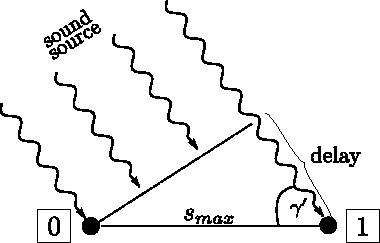
\includegraphics[width=0.4\columnwidth]{figures/tdoa_waves}
	\caption{Illustration of TDOA principle.}
    \label{fig:02_tdoa}
\end{figure}
% -------------------------------------------------------------

Specifying the speed of sound $c_s$ being 343\si{m/s} in air, the angle
$\gamma'$ can be defined as
\bsub \bal
    \gamma' &= cos^{-1}(\frac{|delay|}{s_{max}})
    \label{eq:02_tdoaAngle}\\
    \intertext{with}
    s_{max} &= \frac{f_s * d_{max}}{c_s}
\eal \esub
where $f_s$is the sampling rate.
% -------------------------------------------------------------

With the definition of a whistle signal as stated in \cref{eq:02_whistleSignal},
the microphone sensors $mic_0$ and $mic_1$ will output
\bsub \bal
    x_0(t) &= s(t) + n_0(t)\\
    x_1(t) &= \alpha s(t - D) + n_1(t).
\eal \esub
\label{eq:02_signalTimeDomain}
Here, $D$ is the delay of $x_1$ relative to $x_0$ for which is looked for.